\documentclass{beamer} %for at du kan lave en pr�sintation skal du skriove beamer i class% 
\usetheme{Marburg} %her bestemmer du designet fx madrig du kan ogs� bestemme om der skal vises under katagorier%
\setcounter{tocdepth}{1}

\usepackage[latin1]{inputenc} %standart%
\usepackage[english]{babel}%standrat%
\usepackage{amsmath,amsfonts,amssymb}%standrat%
\usepackage[]{subfig}
\usepackage[]{tabularx}
\usepackage[]{graphicx}
\usepackage{movie15}
\usepackage{tikz} 
%\usepackage{media9}

\usepackage{listings}


\usepackage{color}

\newcommand{\titlename}{Implementering af Aalborg Modellen for Problembaseret L�ring i Moodle}

\definecolor{light-gray}{gray}{0.80}
\definecolor{gray95}{gray}{.95}
\definecolor{gray92}{gray}{.92}
\definecolor{gray75}{gray}{.75}
\definecolor{gray45}{gray}{.45}
\definecolor{darkgreen}{rgb}{0.0,0.7,0.0}

\lstdefinestyle{sourceCode}
{ 
	numbers=left,
	numbersep=5pt, 
	stepnumber=1,
	captionpos=b,  %bottom
	keywordstyle=\color[rgb]{0,0,1},
	commentstyle=\color[rgb]{0.133,0.545,0.133},
	stringstyle=\color[rgb]{0.627,0.126,0.941},
	%backgroundcolor=\color{gray95},
	%frame=lrtb,
	framerule=0.5pt,
	linewidth=1.00\textwidth,
	tabsize=4,
	numberbychapter=true,
	basicstyle=\ttfamily\footnotesize,
	language=C,
	breaklines=true,
	showstringspaces=false,
	emph=[1]{endregion,region,get,set,enum},%%%%%%%%%%% Add new keywords here
	%emph=[2]{Tag,Problem,Person,List,NotSupportedException,TestMethod,ProblemSearch,Assert,
	%EntityCollection,Department,IEnumerable,TimeSpan,DateTime},%%Classes
	emphstyle=[1]{\color[rgb]{0,0,1}},
	emphstyle=[1]{\color[rgb]{0,0,1}},
	emphstyle=[2]{\color[rgb]{0.1,0.5,0.5}},
	float=htb,
	breakindent=20pt
}






\author{SW608F12}
\institute{Aalborg University}
\title{\titlename}
\subtitle{Applikantionsudvikling}


\begin{document}
	\begin{center}
	\parbox{\textwidth}{
		\begin{center}

			\thispagestyle{empty}

			\LARGE
			AALBORG UNIVERSITY \\


			STUDENT REPORT \\
			sw608f12 \\ 
			
			\vspace{10mm}
			
			\begin{figure}[H]%
			\centering
			\LARGE
			\begin{tabular}{ c }
			\hline \\
				\textbf{Implementing the} \\
				\textbf{Aalborg Problem Based Learning Model} \\ 
				\textbf{in Moodle} \\ \\
			\hline 
			\end{tabular}
			\end{figure}

			Theme: \\
			Application Development \\
			 
			\vspace{10mm}
			Authors: \\
			Alex Bondo Andersen\\
			Kim Ahlstr\o{}m Jakobsen\\
			Mikael Midtgaard\\
			Rasmus Veiergang Prentow\\ 
			
			
		
			

		\end{center}		
	}
\end{center}
	
	\chapter{Introduction}
\label{chap:introProjectgroup}
As of this chapter ``we'' only refers to the four authors of this report, and not the 14 collaborators of this project.

As defined in \secref{sec:problemDef} this project is concerned with integrating the Aalborg PBL model into Moodle.
An important concept of this model is the ``Team'' (see \secref{sub:aaupbl}).
For a team to operate in an interactive environment it is necessary to have some entity that defines the members of the team and the actions that they can perform to solve their problem.
We call this entity a ``Project Group''.

To make \system{} usable at any educational institution we provide some form of administrative tool to manage project groups -- e.g. allowing  creation, modification, and archiving of project groups.
The members of the project group will have access to some shared activities through which they can conduct they group work.
These activities include planning the course of the project, communicating internally during the course of the project, and communicating with people not actively part of the project group, such as supervisors (se mentioned \secref{sub:decomposingSys}).
These activities are created in our peer sub-projects.
Our responsibility is to make all these activities available to the members of the project groups.

	\newcommand{\reqs}{Systemkrav}
\newcommand{\slutbrugere}{Slutbrugere}
\newcommand{\funcreqs}{Funktionelle}
\newcommand{\nonfuncreqs}{Ikke-Funktionelle}
%\newcommand{\nonfuncreqs}{Kvalitetskrav}

\newcommand{\admreq}{Administration af Projektgrupper}
\newcommand{\virtgrproomreq}{Det Virtuelle Grupperum}
\newcommand{\rolereq}{Rollebegreb}
\newcommand{\findgrpreq}{Find Projektgruppe}
\newcommand{\navreq}{Navigation til Virtuelt Grupperum}
\newcommand{\grpmemreq}{Pr�sentation af Gruppemedlemmer}


\section{\reqs}
\begin{frame}{\reqs}
	\begin{itemize}
		\item System baseret p� krav
		\item<2-> Krav kommer fra slutbrugere
	\end{itemize}
\end{frame}



\begin{frame}{\reqs}{\slutbrugere}
	\begin{itemize}
		\item Kategorier
		\begin{itemize}
			\item Brugere af projekt grupper
			\item Managere af projekt grupper
		\end{itemize}
		\item Dimensioner
		\begin{itemize}
			\item Type
			\item Fakultet
			\item Institut
			\item LMS erfaring
		\end{itemize}
	\end{itemize}
\end{frame}

\begin{frame}{\reqs}{\slutbrugere}
	\begin{itemize}
		\item Brugere af projekt grupper
	\end{itemize}
	\begin{figure}
		\centering
			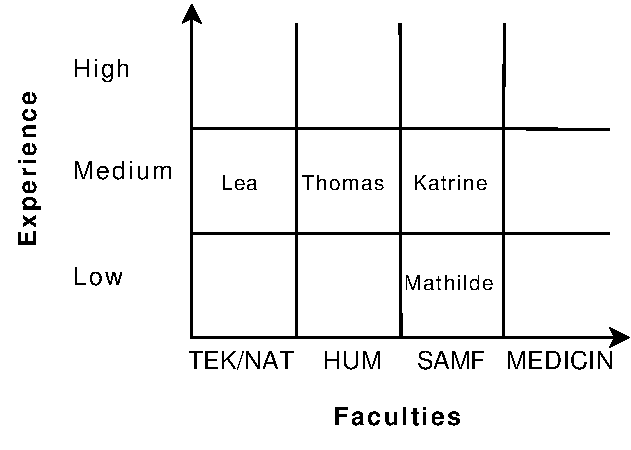
\includegraphics[width=\textwidth]{../report/images/MembersofpROJECTgROUJP.pdf}
		\label{fig:MembersofpROJECTgROUJP}
	\end{figure}
\end{frame}

\begin{frame}{\reqs}{\slutbrugere}
	\begin{itemize}
		\item Managere af projekt grupper
	\end{itemize}
	\begin{figure}
		\centering
			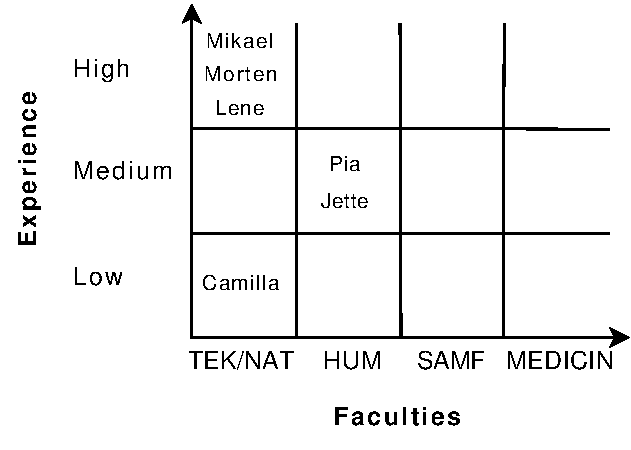
\includegraphics[width=\textwidth]{../report/images/administratorsOfPG.pdf}
		\label{fig:administratorsOfPG}
	\end{figure}
\end{frame}



\newcommand{\chosenreqs}[1]{\begin{columns}[t]
		\column{0.45\textwidth}
			\begin{itemize}
				\item \textcolor{#1}{Administrering af Projektgrupper}
				\item \textcolor{#1}{Det Virtuelle Grupperum}
				\item \textcolor{#1}{Rollebegreb}
			\end{itemize}
			
			
		\column{0.45\textwidth}
			\begin{itemize}
				\item \textcolor{#1}{Find Projektgruppe}
				\item \textcolor{#1}{Naviger til Virtuelt Grupperum}
				\item \textcolor{#1}{Pr�senter Gruppemedlemmer}
			\end{itemize}
	\end{columns}}
	
\begin{frame}{\reqs}{\funcreqs}
	\begin{itemize}
		\item \admreq
		\item \virtgrproomreq
		\item \rolereq
		\item \findgrpreq
		\item \navreq
		\item \grpmemreq
	\end{itemize}
	%Chosen
	%\only<1>{
		%\chosenreqs{black}
		%}
	%\only<2>{
		%\chosenreqs{darkgreen}
	%}
	%%Not chosen
	%\begin{columns}[t]
		%\column{0.45\textwidth}
			%\begin{itemize}
				%\item Arkivering af projektgrupper
				%\item Rekursive Projektgrupper
				%\item Administrer Roller
			%\end{itemize}
			%
		%\column{0.45\textwidth}
			%\begin{itemize}
				%\item Synkronisering af Projektgrupper
				%\item Skabeloner for Virtuelle M�desteder
			%\end{itemize}
		%
	%\end{columns}
	
\end{frame}

\begin{frame}{\reqs}{\nonfuncreqs}
	\begin{itemize}
		\item Udvidbarhed
		\item Robusthed
		\item Brugbarhed
	\end{itemize}
\end{frame}







	
	
	\section*{Udviklingsmetode}

\begin{frame}{Udviklingsmetode}{Udviklingsparadigme}

\begin{itemize}
	\item 
\end{itemize}

\end{frame}
%%%%%%%%%%%%%%%%%%%%%%%%%%%%%%%

\begin{frame}{Udviklingsmetode}{Valg af Agil Udviklingsmetode}



\end{frame}
%%%%%%%%%%%%%%%%%%%%%%%%%%%%%%%

\begin{frame}{Udviklingsmetode}{Tilpasning af Udviklingsmetode}
	
\end{frame}
%%%%%%%%%%%%%%%%%%%%%%%%%%%%%%%

\begin{frame}{Udviklingsmetode}{Evaluering af Udviklingsproces}
	
\end{frame}

  \newcommand{\modelreality}{Virtuelt Grupperum}
\newcommand{\topicone}{Aalborg PBL}
\newcommand{\topictwo}{Repr\ae{}sentation}
\newcommand{\topicthree}{Eksempel}
\newcommand{\topicfour}{Design}

\newcommand{\implementaras}{\modelreality}
\newcommand{\topictwoe}{Valg af Plugin Typer}
\newcommand{\topicthreee}{Context}

\section*{\modelreality}

\begin{frame}{\modelreality}
\begin{itemize}
	\item Analyse
	
	\begin{itemize}
		\item \topicone
		\item \topictwo
  \end{itemize}
	
	\item \topicfour
	\begin{itemize}

		\item \topictwoe
		\item \topicthreee
	\end{itemize}
	\item Implementation
  \begin{itemize}
		\item Standard Projekt V�rkt�jer
	\end{itemize}

\end{itemize}
\end{frame}

\begin{frame}{\modelreality}{Analyse} 

\begin{center}
\huge Analyse
\end{center}

\end{frame}

\begin{frame}{\modelreality}{\topicone}
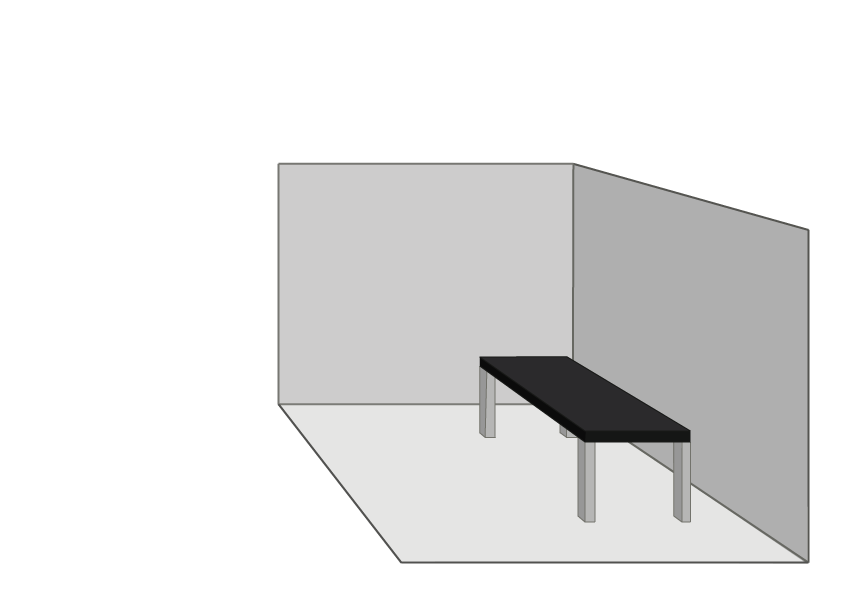
\includegraphics[width=\columnwidth]{input/rasmus/ras5.png}
\end{frame}
\begin{frame}{\modelreality}{\topicone} 
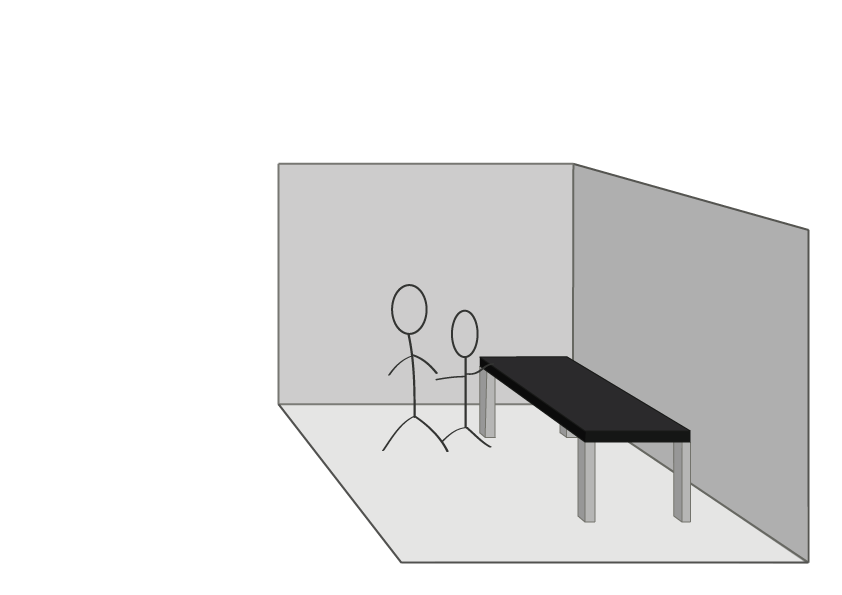
\includegraphics[width=\columnwidth]{input/rasmus/ras4.png}
\end{frame}
\begin{frame}{\modelreality}{\topicone} 
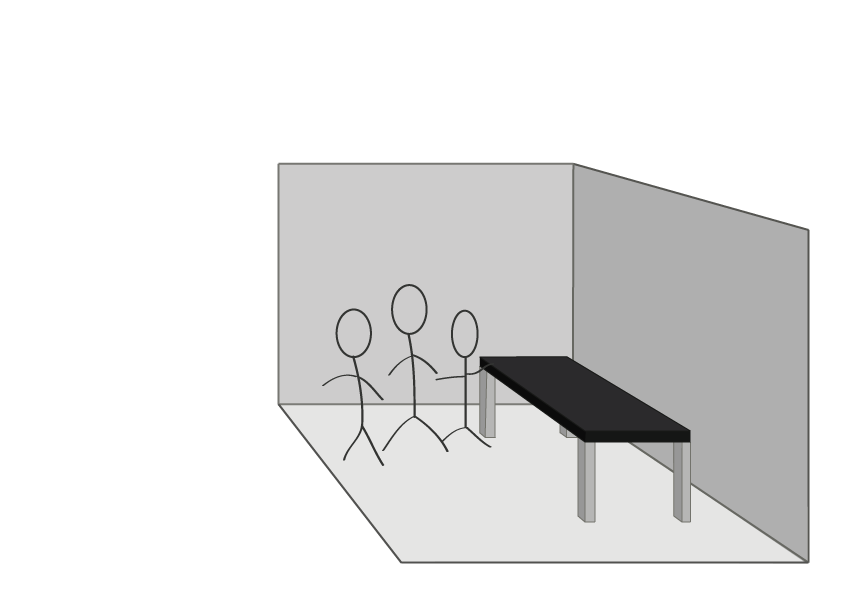
\includegraphics[width=\columnwidth]{input/rasmus/ras3.png}
\end{frame}
\begin{frame}{\modelreality}{\topicone} 
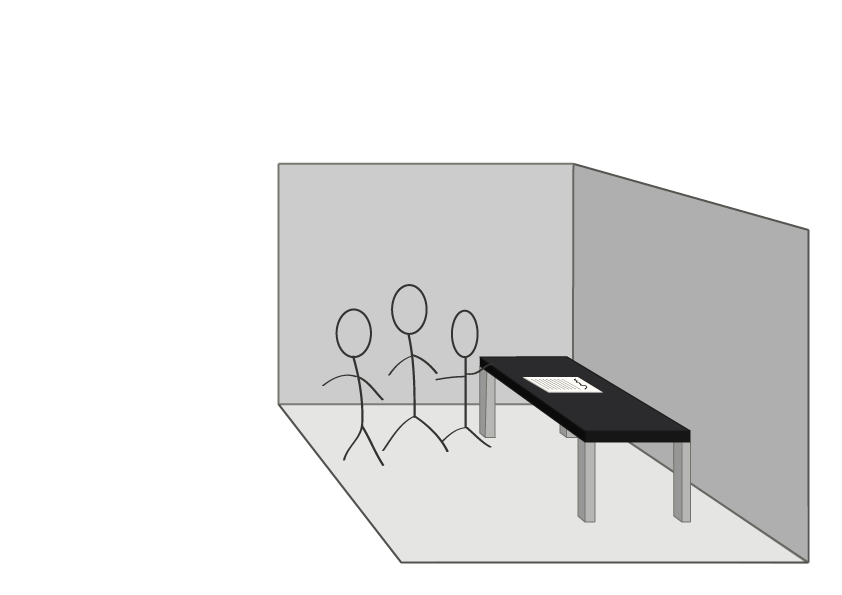
\includegraphics[width=\columnwidth]{input/rasmus/ras2.png}
\end{frame}
\begin{frame}{\modelreality}{\topicone} 
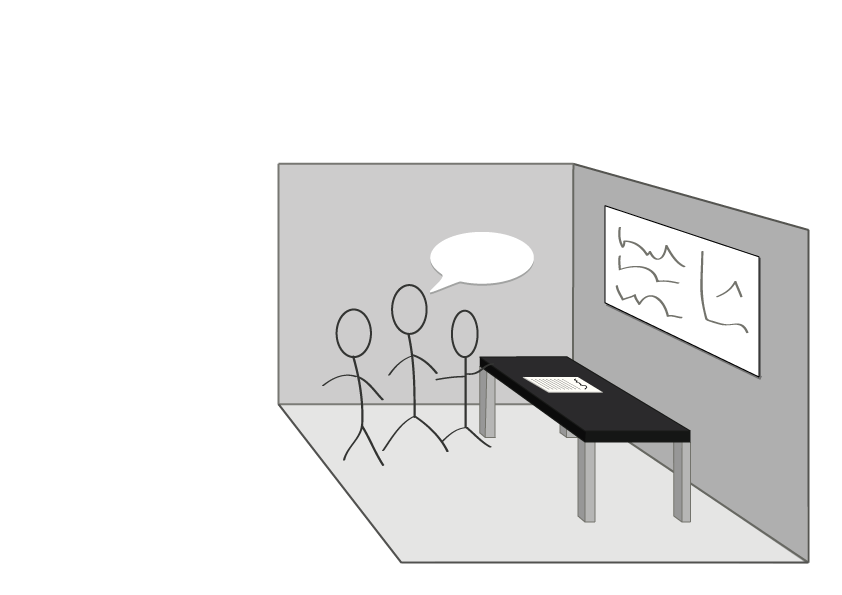
\includegraphics[width=\columnwidth]{input/rasmus/ras1.png}
\end{frame}


\def\freqlist{1,2,3}

\foreach \freq in \freqlist 
{
\begin{frame}{\modelreality}{\topictwo} 
\begin{figure}
\includegraphics[width=\columnwidth]{input/rasmus/two\freq.pdf}
\end{figure}
\end{frame}

} 

\def\freqlist{4,5,6}

\foreach \freq in \freqlist 
{
\begin{frame}{\modelreality}{\topicthree} 
\begin{figure}
\includegraphics[width=\columnwidth]{input/rasmus/two\freq.pdf}
\end{figure}
\end{frame}

} 

\def\freqlist{7,8,9}

\foreach \freq in \freqlist 
{
\begin{frame}{\modelreality}{\topictwo} 
\begin{figure}
\includegraphics[width=\columnwidth]{input/rasmus/two\freq.pdf}
\end{figure}
\end{frame}

} 

\begin{frame}{\modelreality}{\topicfour} 

\begin{center}
\huge Design
\end{center}

\end{frame}


\begin{frame}{\modelreality}{\topicfour} 
\begin{figure}
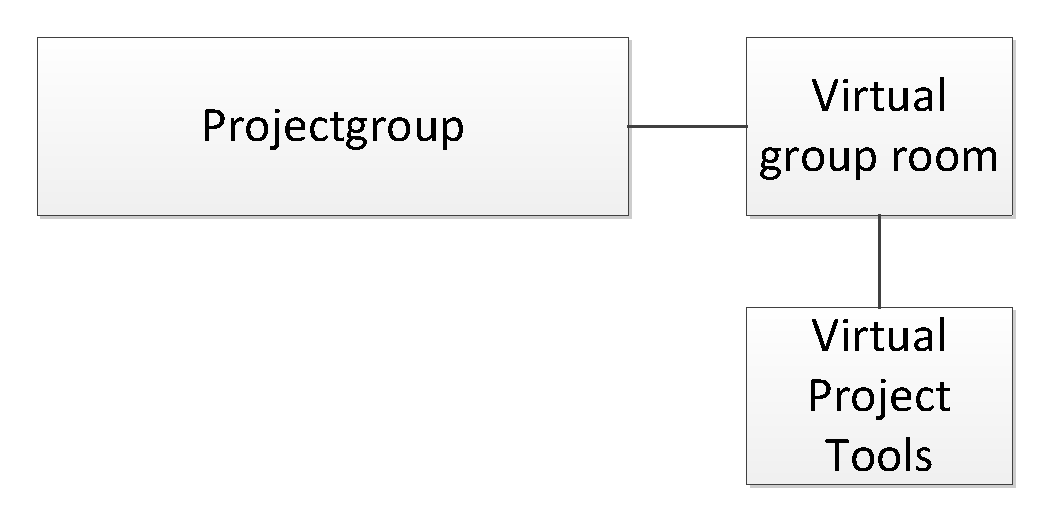
\includegraphics[width=\columnwidth]{input/rasmus/two10.pdf}
\end{figure}
\end{frame}

\begin{frame}{\modelreality}{\topicfour} 
\begin{figure}
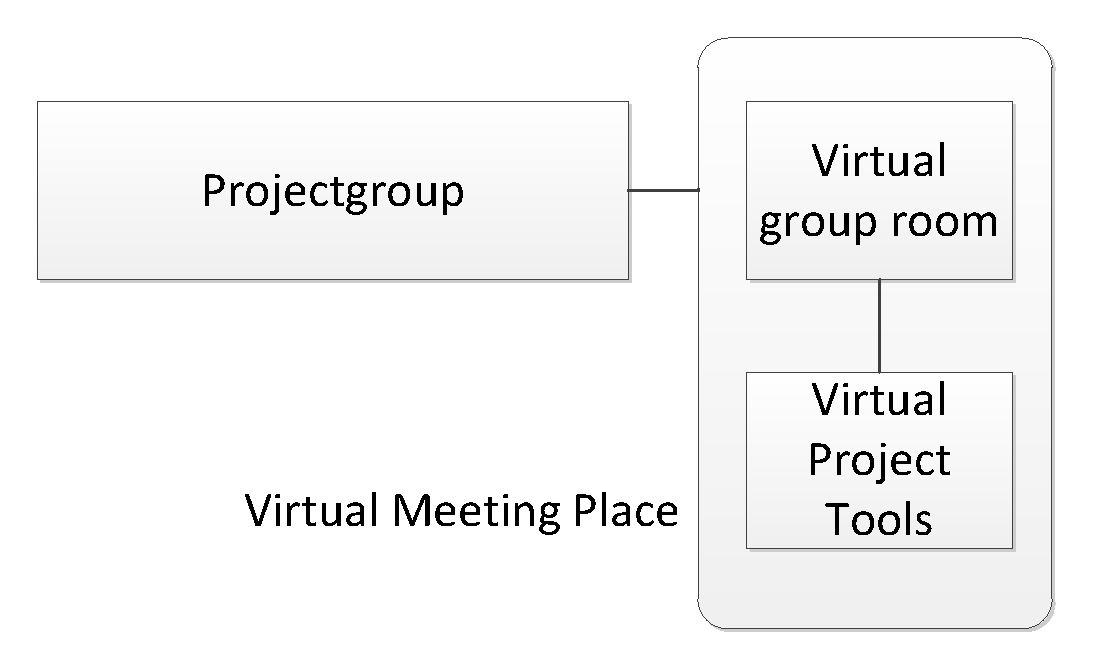
\includegraphics[width=\columnwidth]{input/rasmus/two11.pdf}
\end{figure}
\end{frame}



\def\freqlist{1,1a,2,3,4,5,6,7,7a,8}

\foreach \freq in \freqlist 
{
\begin{frame}{\implementaras} {\topictwoe}
\begin{figure}
\includegraphics[width=\columnwidth]{input/rasmus/three\freq.pdf}
\end{figure}
\end{frame}
}

\def\freqlist{9}

\foreach \freq in \freqlist 
{
\begin{frame}{\implementaras}{\topicthreee} 
\begin{figure}
\includegraphics[width=\columnwidth]{input/rasmus/three\freq.pdf}
\end{figure}
\end{frame}
} 


\begin{frame}{\implementaras}{\topicthreee}
\begin{figure}
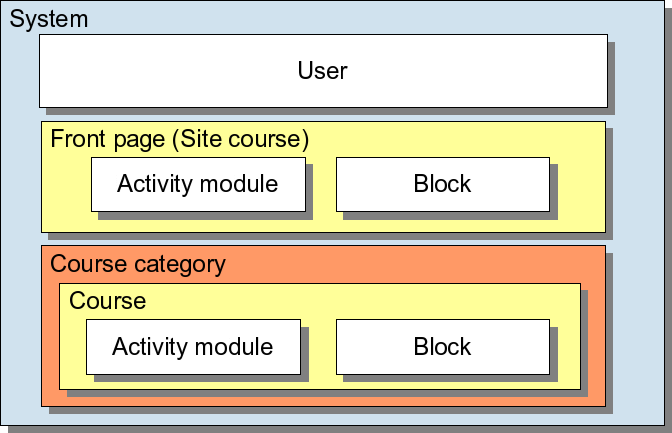
\includegraphics[width=\columnwidth]{input/rasmus/Moodle-contexts.png}
\end{figure}
\end{frame}

\begin{frame}{\implementaras}{\topicthreee}
\begin{figure}
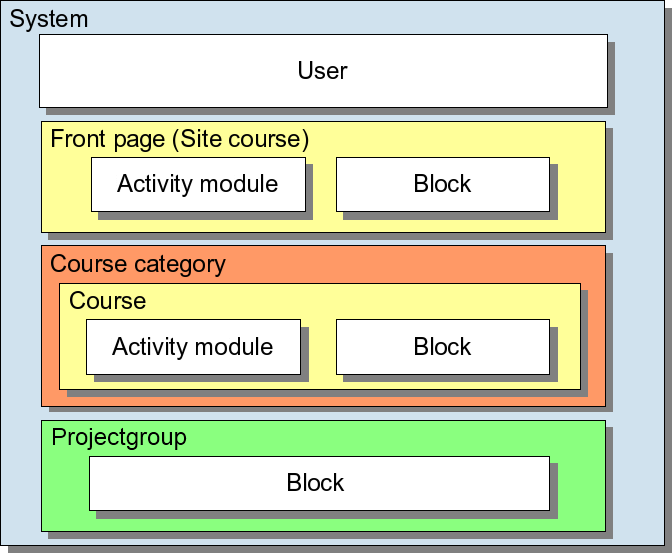
\includegraphics[width=\columnwidth]{input/rasmus/Moodle-contexts-mymoodle.png}
\end{figure}
\end{frame}


\begin{frame}{\modelreality}{Implementation} 

\begin{center}
\huge Implementation
\end{center}

\end{frame}
	
	
	\section{Architecture}
\label{sec:architecture}
\system{} is an extension of \moodle{} and can be seen as a package of plugins. 
The architecture does not specify how each plugin should be created, but specifies a general structure of the components of the system. 
The complete architecture can be seen in \figref{fig:architecture}.
\begin{figure}[h!t]
	\centering
		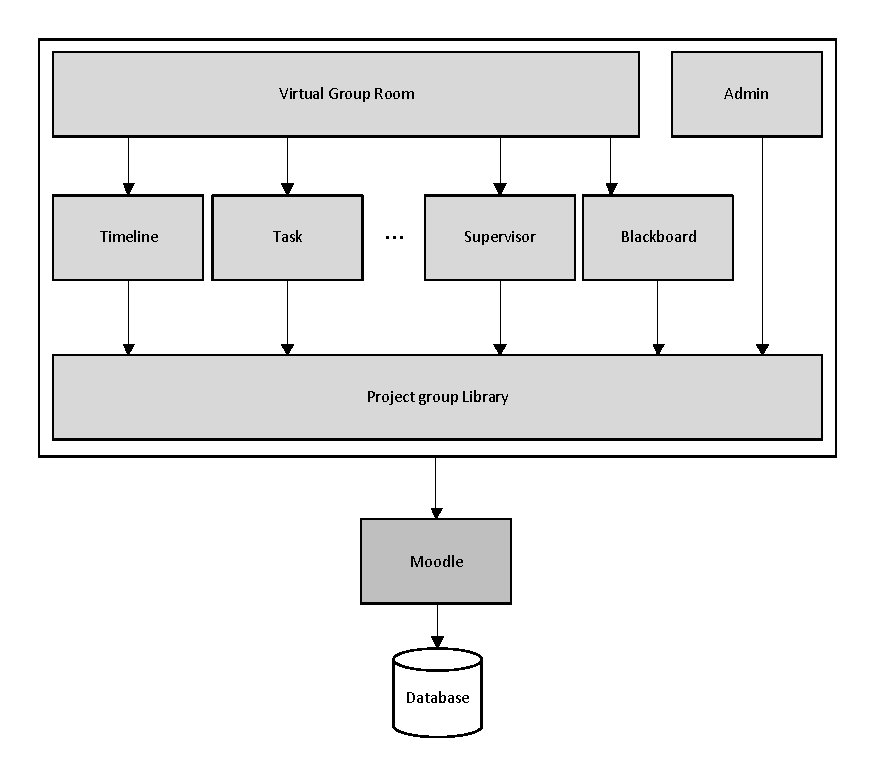
\includegraphics[width=\textwidth]{images/architecture.pdf}
	\morscaption{The overall architecture of MyMoodle}
	\label{fig:architecture}
\end{figure}

The architecture consists of a total of five layers. 
The three uppermost constitute \system{}, they have a common dependency, namely the Moodle platform. 
Layers four and five are Moodle and the Database system respectively.
%Our extension  as a plugin of Moodle and use functions supplied by Moodle to function.

We explain the three uppermost layers as:
\begin{enumerate}
	\item The uppermost layer is the virtual group room and the administration tool.
	%The virtual group room is used for presenting the virtual meeting place for a project group.
	The virtual group room is described in \secref{sec:virtualMeetingPlace}.
	The administrative tool is used by administrative personnel for managing project groups.
	It is described in \secref{sec:groupManagement}.
	This layer is called ``View Layer''.
	\item Directly below the uppermost layer is the middle layer, which consists of the four components: Timeline, Task, Supervisor, and Blackboard.
	These four components are created by our peer-groups and are not explained further.
	We call this layer ``Content Layer'', since the components in this layer generate content for the virtual group room component.
	This layer has three dots in the center in order to show that there exist more components and more can be added here. 
	%An example is the \detdeandrelaver{} that presents the members of the project group. 
	\item Below the Content Layer is the project group library, which contains common functionality.
	This layer handles all communication between the components in the Content Layer.  
	We call this layer the ``Library Layer''.
\end{enumerate}


There are two primary factors we need to consider when planning our architecture. 
Firstly, we are four sub-groups working together. 
This creates the need for a structured way of communicating between the different component and it lets every \subgroup{} know how their component is connected to the rest of the project. 
Secondly, the project should be passed on, which requires an architecture that grants great comprehensibility and extensibility of the project.
%alex -> <@:-D-|-<

It is not possible to make a strict layered architecture due to the Moodle dependency, and the administrative tool, which does not have to use the Content Layer, but depends directly on the project group library and \moodle{}.
We do, however, prohibit ourselves from accessing the database directly, by using the Moodle Database Layer (note that it is not a layer in our architecture) described in \secref{sec:moodleoplatformdbml}.
In \figref{fig:architecture} the dependency from the box encircling \system{} indicates that every component in \system{} depends on the \moodle{} component.
The \moodle{} component consists of the Database Layer as well as the Context System, Capabilities, etc.

%These considerations leads us to design the illustrated architecture in \figref{fig:architecture}.
Note that the relative size of the components do not imply anything, e.g.\ the Moodle component is code wise much larger, than all of the components in \system{} combined, but is illustrated with a rectangle the same size as any of the Content Layer components.













	\chapter{Implementation}
\newcommand{\viewroom}{}
\myTop{In this chapter we describe how we implement the concepts described in \secref{chap:design}.
%This chapter is divided into three sections where the two main parts of our system are described, namely \nameref{sec:projGroupRoomImpl} and \nameref{sec:manProjGrpImpl}.

The implementation details presented here are paramount for \chapref{chap:test} and \chapref{chap:evalProduct}.}
From section \secref{sec:architecture} we know there is three part which must be implemented by us. 
The administration tool to manage project group, the project group, and the project group \viewroom. 
The administration tool is implemented as an admin tool, which as described in \section{platform} is a special moodle plugin type. 
Project groups can be implemented as courses (see \secref{sub:courses}) by creating a new view for the course page. 
Hereby solving the problem of both implementing project groups and the aforementioned project group \viewroom.
This will make it possible to use activity modules, described in \ref{par:activitymodules}, in the project group. 
Another approach is to make a local plugin, which gives us basic functionality, such as database installation. 
With a local plugin we cannot use activity modules since they are too strongly connected to courses. 
Instead we can use blocks for the functionality. 
The later approach is chosen. 
The local plugin includes both the project group library and the project group  \viewroom. 
The view is implemented in the file \moodlefile{/local/projectgroup/view.php} and  the library is in the file \moodlefile{/local/projectgroup/lib.php}. 
The library includes several other files. 
One for each sub group and several helper files. 

\section{Project group library}
The project group library is build up by several files and consist of several functions and classes.
It is shared between all subgroups. 
This section only explains the functionality implemented by our subgroup. 
%% Lines of codes
%% How many functions

In the following sections is how we put our project group into a moodle context and how we ensure permissions.

\subsection{Overwrite Context}
In \secref{sub:contextsystem}  the context system of Moodle is described.
In this section the creation of a custom context is described. 

To be able to define capabilities for the project groups and have different blocks for different project group we need our own context.
We will create our own context level and class.
We call the context \cl{context\_projectgroup}. 

Moodle does not support extension of contexts through one of the more than 30 different plugin types available \cite{plugin}. 
There two parts of the problem, the first is to create a new context and the second is to load it properly. 
We create a new context by making a new class which is very similar to \cl{context\_course} class and by defining the context level of project groups as a constant. 
The class header and the constant definition can be seen in \coderef{codeprojectgroupcontext}. 
The constant is set to 55 and is chosen because that context level is unused and it is close to the course context level. 
We regard the project group contexts to be at the same level as course contexts. 
However, project groups does not have categories like courses does.

\begin{lstlisting}[style=phpCode, caption=\myCaption{The context\_projectgroup class header and constant definition}, label=codeprojectgroupcontext]
define ('CONTEXT_PROJECTGROUP',55);
class context_projectgroup extends context {
...
\end{lstlisting}

When a context is loaded in a Moodle page it is instantiated by \fu{get\_context\_instance}, which takes a context level and an instance id. 
The instance id can be a course id or similar depending on the context level -- in our case it is a project group id. 
This function calls a static method in the \cl{context\_helper} class which uses a private array to translate the context level into a class name.
The overall system definition in \chapref{chap:systemDef} retain us from changing the core code of Moodle. 
If this constraint were not enforced the array could simply be extended directly in the code.  
Since the array used is private we can not extend the context system by overriding the \cl{context\_helper} class. 
The newly created context is only used in pages created in this project and we can therefore create our own version of \fu{get\_context\_instance}. 
The new function can be seen in \coderef{codeprojectgroupcontextinstance}.
\begin{lstlisting}[style=phpCode, caption=\myCaption{The function to get projectgroup context}, label=codeprojectgroupcontextinstance]
function get_projectgroup_context_instance( $instance = 0, $strictness = IGNORE_MISSING) 
{ 
    return context_projectgroup::instance($instance, $strictness);
}
\end{lstlisting}
The \vari{instance} variable denotes a project group id.
The \vari{strictness} variable 

With the new context and the function to instantiate it we can now make per project group permissions and add blocks to specific project group pages. 
\subsection{Ensuring Permissions}
\label{sec:projectgrouproommanagerights}
Permissions can generally be divided in two types; read and write. 
Read permissions gives you the ability to view the content of the virtual group room while write lets you change the content. 
If a user has write permission he must also have read permissions, otherwise he cannot see the page he attempts to edit. 
To ensure the user attempting to enter a virtual group room has permission to enter the function \fu{has\_projectgroup\_read\_permission} is used. 
%It checks if the user is a member of the group. 
It checks if the user is an administrator or is a member of the project group. 
The administrator check is necessary since an administrator should be able to see any project group even if he is not a member of the project group. 

The function \fu{has\_projectgroup\_write\_permission} checks that the user has write permissions and uses the read permission function to check that the user has read permission.
If he does not have read permission he should not be able to edit the virtual group room. 
In the current implementation the write permissions function does not make extra checks to permissions since the permission levels for read and write are equivalent.

Because the functions are separate it is possible to change them individually later.
%Making both function gives the ability to later change this.
An example is that an end users requires that supervisors should only have read permissions. Then the change will only be in one place. 
Both functions can be found in the project group library.


\FloatBarrier

In the implementation of the project group we are faced with several choices. 
Project groups can be implemented as courses by creating a new view for the course page.  
This will make it possible to use activity modules, described in \ref{par:activitymodules}, in the project group. 
Another approach is to make a local plugin, which gives us basic functionality, such as database installation. 
With a local plugin we cannot use activity modules since they are too related to courses. 
Instead we can use blocks for the functionality. 
The later approach is chosen. 

\section{Project Group Room}
In this section the actual implementation of the project group room, its custom blocks, how the context system is used to implement our own context to allow better administration of blocks and capabilities, and the navigation to the users project groups is described.
The section presents how the project groups work from the perspective of the user. 


\subsection{The page}
The project group page is the virtual meeting place described in \secref{sec:projectgroup}.
We decided to implement the room merely as a container for blocks. 
Alternatively the functionality could be an integrated part of the page, but using blocks gives more flexibility to the users allowing them manage the layout of their own project group room. 
A screenshot of a project group room can be seen in \figref{fig:projectgroupnoedit}. 
In this project group room the blocks are layouted as they are per default. 
\begin{figure}[h]
	\centering
		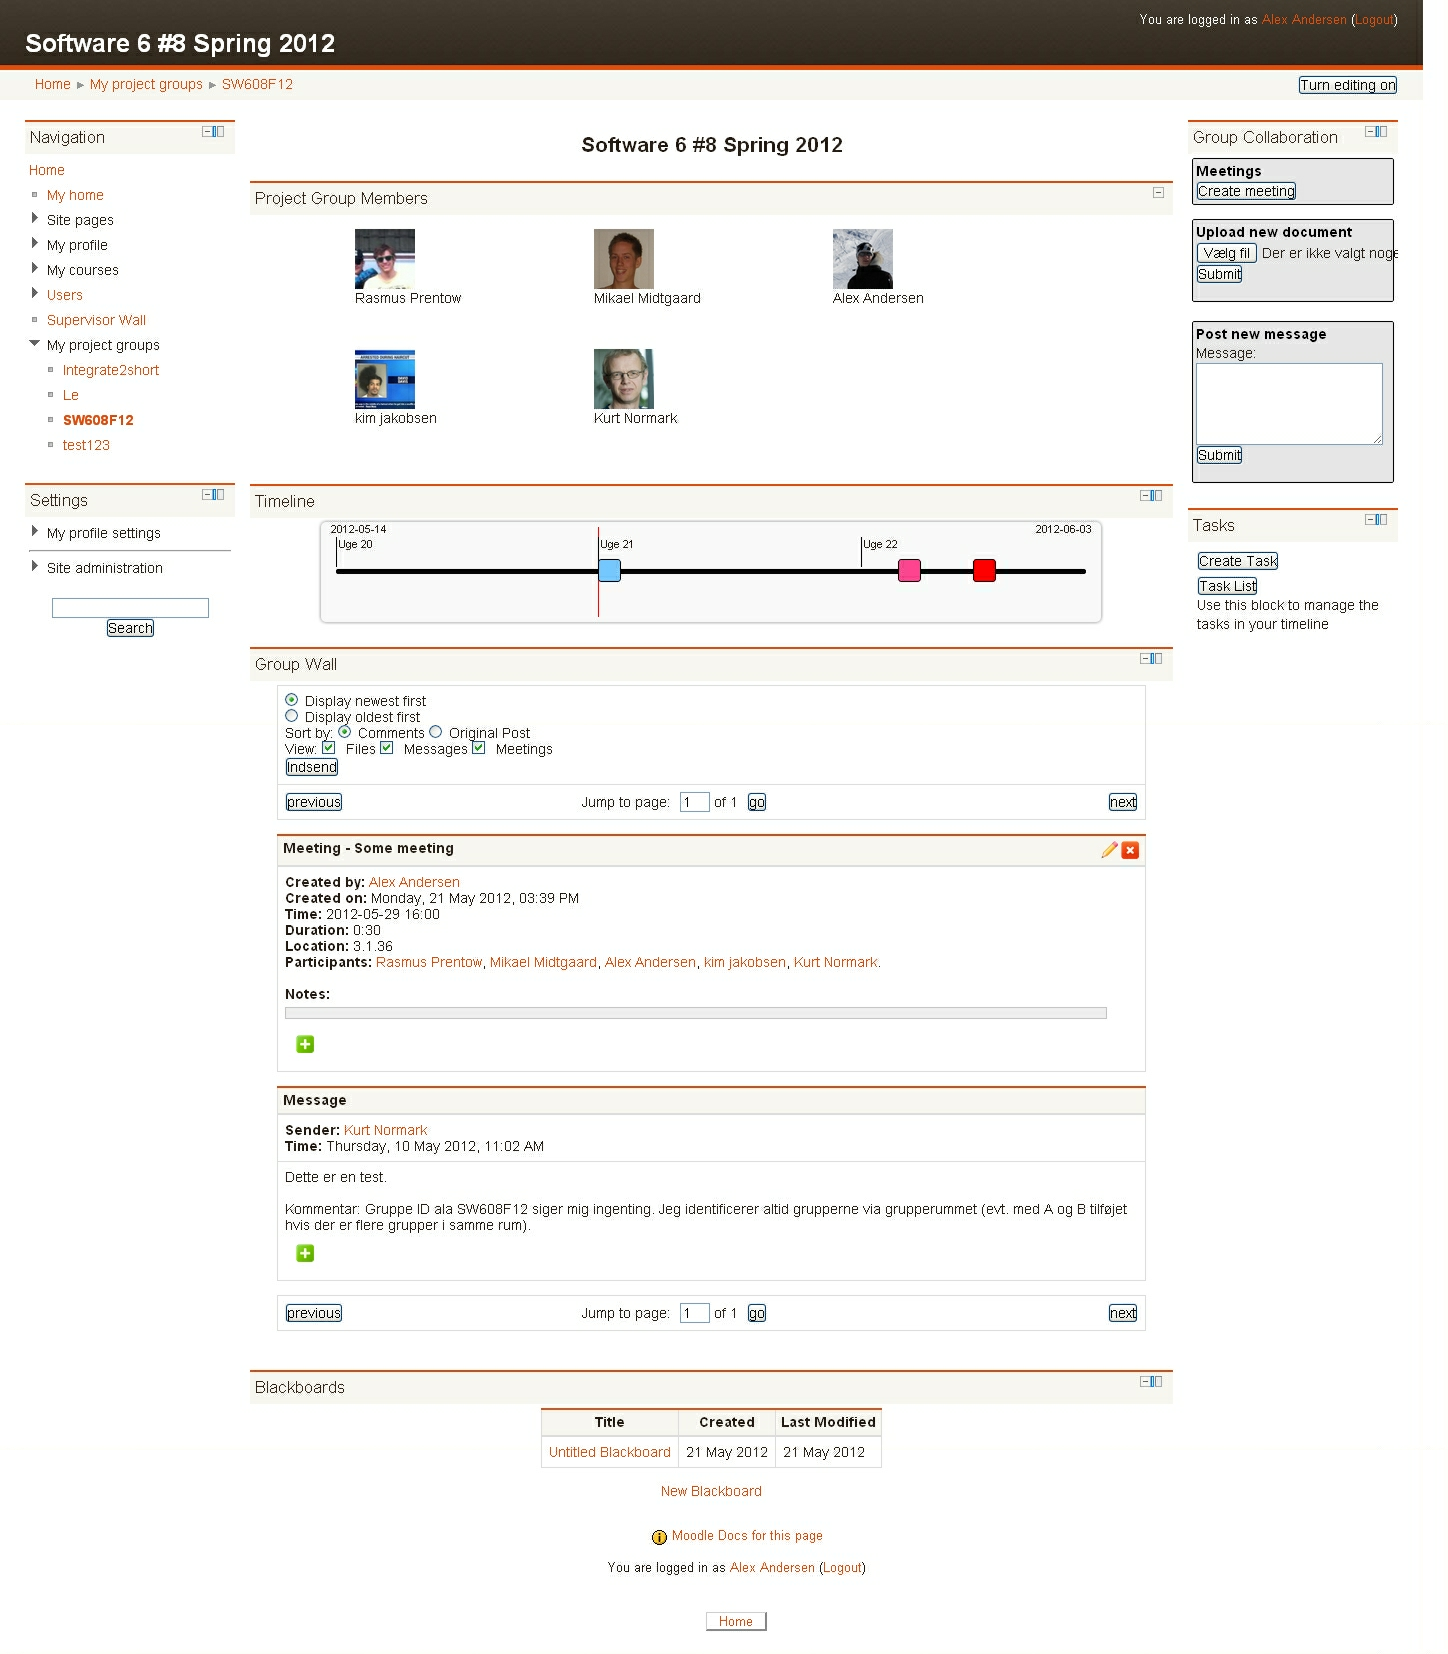
\includegraphics[width=\textwidth]{images/projectgroupnoedit.png}
	\morscaption{The project group room}
	\label{fig:projectgroupnoedit}
\end{figure}

The project group room consist of three columns. 
The left column is the standard navigation menu in Moodle. 
The Center and right columns both contain blocks.
The various blocks presented on the project groups page is described in \secref{sec:implprojectgroupblocks}. 
If an user wants to edit the block layout for the project group room he can press the ``Turn editing on'' button. 
This will add edit and move buttons to each block. 
A new block is added in editing mode to allow for adding new blocks. 
If an user edits the page the change can be seen by all group members. 
The page in edit mode can be seen in figure \figref{fig:projectgroupwithedit}.

\begin{figure}[h]
	\centering
		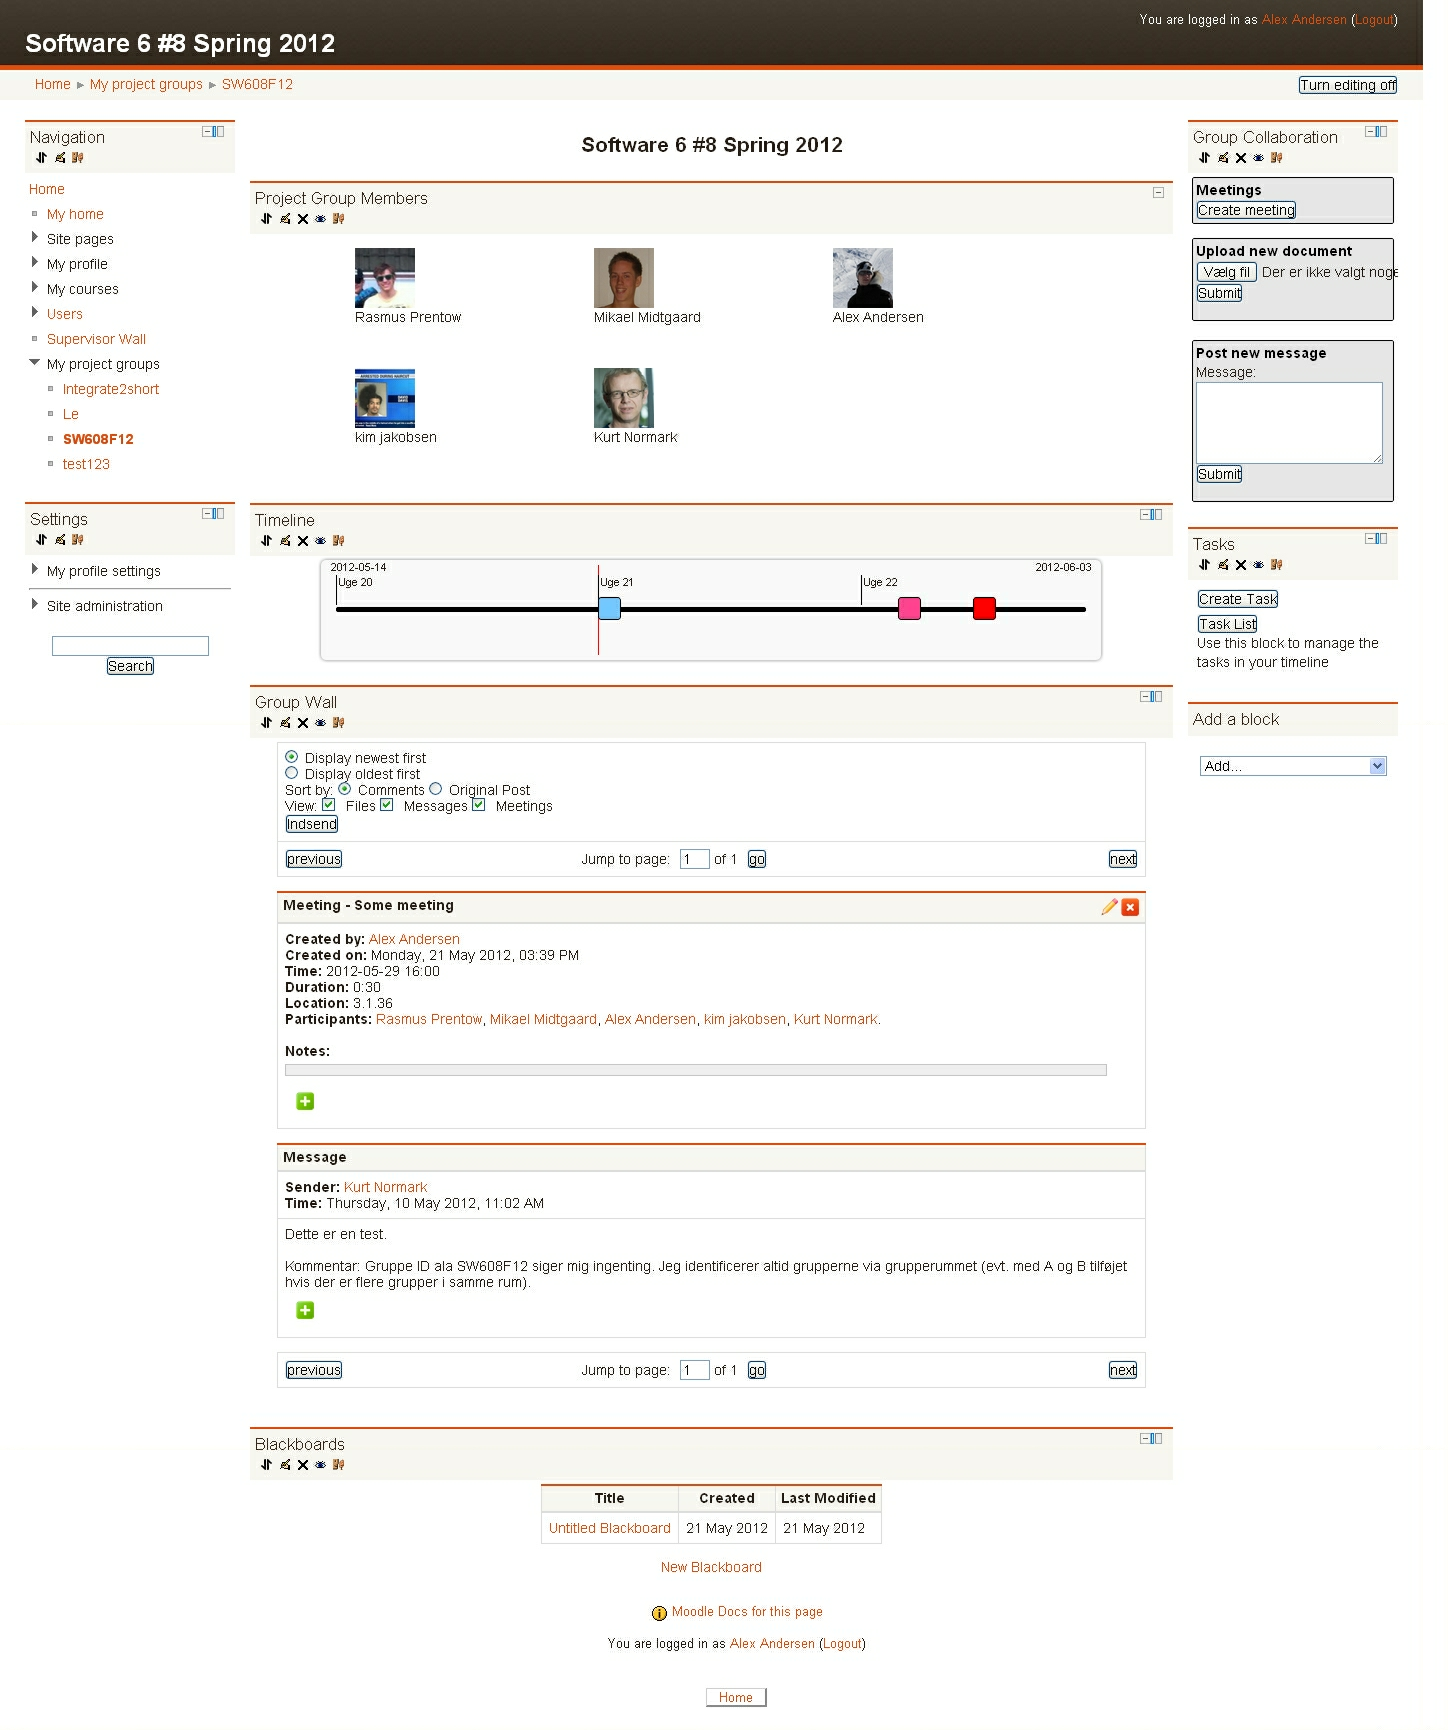
\includegraphics[width=\textwidth]{images/projectgroupwithedit.png}
	\morscaption{The project group room with editing turned on}
	\label{fig:projectgroupwithedit}
\end{figure}


The task of securing that only members of the project group can edit and view are maintained by the project group room and is described in \secref{sec:projectgrouproommanagerights}. 




\subsection{Ensuring Permissions}
\label{sec:projectgrouproommanagerights}
Permissions can generally be divided in two types; read and write. 
Read permissions gives you the ability to view the content of the project group room while write lets you change the content. 
If a user has write permission he must also have read permissions. 
Otherwise he cannot see the page he attempts to edit. 
To ensure the user attempting to enter a project group room has permission to enter the function \fu{has\_projectgroup\_read\_permission} is used. 
It checks if the user is an administrator or is a member of the group. 
The administrator check is necessary since administrators should be able to see the group even if they are not members of the group. 

The function  \fu{has\_projectgroup\_write\_permission} which checks that the user has write permissions uses the read permissions function too check that the user can read.
If he cannot read he should not be able to edit. 
In the current implementation the write permissions function does not make extra checks to permissions since the permission level for read and write is equivalent.
Making both function gives the ability to later change this.
An example could be if the potential users requires that their supervisor should only have read permissions. 
Then the change will be in one place only. 

\subsection{Blocks}
\label{sec:implprojectgroupblocks}
When a new project group is created the default blocks are added to the page. 
The default blocks are specified in the a config file and the content can be seen in \coderef{moodledaultblock}


\begin{lstlisting}[style=phpCode, caption=\myCaption{The default block configuration}, label=moodledaultblock]
<?php
	/**
	* Example usage:
	* "left1,left2:center1:right1"
	* Will add two items to the left, one in the middle, and one to the right
	*/
	$format['defaultprojectgroupblocks'] = ':projectgroup_members,timeline,groupwall,blackboard:upload,tasks';
\end{lstlisting}\begin{comment}$\end{comment}
The syntax for the format is $left:middle:right$. 
Left, middle, and right represent the three columns in the project group room. 
The blocks: Timeline, groupwall, blackboard, upload, and tasks is created by our peer-groups while the block named projectgroup\_members is created by us. 
The projectgroup\_members block shows the name and pictures of the project group members. 

	
	


\subsection{Overwrite Context}
In \secref{sub:contextsystem}  the context system of Moodle is described.
In this section the creation of a custom context is described. 

To be able to define capabilities for the project groups and have different blocks for different project group we need our own context.
We will create our own context level and class.
We call the context \cl{context\_projectgroup}. 

Moodle does not support extension of contexts through one of the more than 30 different plugin types available \cite{plugin}. 
There two parts of the problem, the first is to create a new context and the second is to load it properly. 
We create a new context by making a new class which is very similar to \cl{context\_course} class and by defining the context level of project groups as a constant. 
The class header and the constant definition can be seen in \coderef{codeprojectgroupcontext}. 
The constant is set to 55 and is chosen because that context level is unused and it is close to the course context level. 
We regard the project group contexts to be at the same level as course contexts. 
However, project groups does not have categories like courses does.

\begin{lstlisting}[style=phpCode, caption=\myCaption{The context\_projectgroup class header and constant definition}, label=codeprojectgroupcontext]
define ('CONTEXT_PROJECTGROUP',55);
class context_projectgroup extends context {
...
\end{lstlisting}

When a context is loaded in a Moodle page it is instantiated by \fu{get\_context\_instance}, which takes a context level and an instance id. 
The instance id can be a course id or similar depending on the context level -- in our case it is a project group id. 
This function calls a static method in the \cl{context\_helper} class which uses a private array to translate the context level into a class name.
The overall system definition in \chapref{chap:systemDef} retain us from changing the core code of Moodle. 
If this constraint were not enforced the array could simply be extended directly in the code.  
Since the array used is private we can not extend the context system by overriding the \cl{context\_helper} class. 
The newly created context is only used in pages created in this project and we can therefore create our own version of \fu{get\_context\_instance}. 
The new function can be seen in \coderef{codeprojectgroupcontextinstance}.
\begin{lstlisting}[style=phpCode, caption=\myCaption{The function to get projectgroup context}, label=codeprojectgroupcontextinstance]
function get_projectgroup_context_instance( $instance = 0, $strictness = IGNORE_MISSING) 
{ 
    return context_projectgroup::instance($instance, $strictness);
}
\end{lstlisting}
The \vari{instance} variable denotes a project group id.
The \vari{strictness} variable 

With the new context and the function to instantiate it we can now make per project group permissions and add blocks to specific project group pages. 



\subsection{Navigation}



























\section{Managing Project Groups} %Jeg skriver kun om admin funktionalitet her -Mikael ~♥
Before any project group can be useful it has to be created first.
Administrators need to have the ability to add, edit, and delete project groups.
The administration tools we provide have to be easy and fast to use, since they potentially have to be used many times.
This section describes how we implemented the administration tools needed to manage project groups.

The features we provide to manage project groups are known as administration tools in Moodle and can be accessed in the site administration menu as seen in \figref{fig:navigation}.

\begin{figure}[htb]
	\centering
		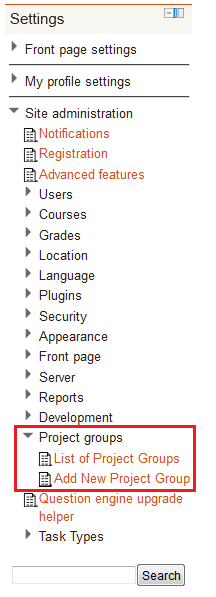
\includegraphics[scale=0.75]{images/admin-navigation.png}
	\morscaption{The settings block, which contains the site administration menu} 
	\label{fig:navigation}
\end{figure}

From here we provide a link to a list of all project groups and a link to a page, from where a new project group can be created.
The page with the list of all project groups has a table with three columns: Short name, Full name, and Actions.
As the name indicates Short name is a short name for a group. 
The Short name also serves as a link to the project group page described in \recref{sub:page}.
In the Actions column there are links to delete and edit the project group.

The edit page has the same source files as the add page.








	
	\section*{Fremtidigt Arbejde}

\begin{frame}{Fremtidigt Arbejde}
	
	\begin{itemize}
		\item something ny folk skal ovetage
	\end{itemize}
	
\end{frame}


\begin{frame}{Fremtidigt Arbejde}
	
	\begin{itemize}
		\item <1-> Booking System
		\item <2-> Skabeloner for Virtuelle Grupperum
		\item <3-> Implementering af V\ae{}rkt\o{}jer
	\end{itemize}
	 
\end{frame}
\end{document}
